%% ===================================================================
%% SEKCE 2.2: KOMPILÁTORY A INTERPRETERY
%% ===================================================================

\subsection{Kompilátory a interpretery}
\label{sec:kompilatory}

Překladač (kompilátor) je program, který transformuje zdrojový kód
napsaný v~jednom programovacím jazyce do jiného jazyka, typicky
do strojového kódu nebo mezikódu \autocite{aho2006}. Tato sekce
poskytuje teoretický základ pro pochopení architektury kompilátoru
\Roth{}.


\subsubsection{Fáze kompilace}
\label{sec:faze-kompilace}

Proces kompilace lze rozdělit do několika oddělených fází, z~nichž
každá provádí specifickou transformaci nad vstupními daty. Moderní
kompilátory typicky implementují následující fáze:

\paragraph{Lexikální analýza (lexer).}
První fáze kompilace převádí vstupní text (proud znaků) na proud
tokenů. Token je základní lexikální jednotka jazyka, například
klíčové slovo, identifikátor, číslo nebo operátor. Lexer ignoruje
bílé znaky a~komentáře (případně je předává jako speciální tokeny).

Pro jazyk \Roth{} rozlišujeme následující typy tokenů:
\begin{itemize}
	\item \texttt{Number} --- celočíselná konstanta
	\item \texttt{Word} --- identifikátor (slovo)
	\item \texttt{StartDefinition} --- znak \texttt{:}
	\item \texttt{EndDefinition} --- znak \texttt{;}
	\item \texttt{StringLiteral} --- řetězcová konstanta
	\item \texttt{Comment} --- komentář v~závorkách
\end{itemize}

\paragraph{Syntaktická analýza (parser).}
Parser převádí proud tokenů na abstraktní syntaktický strom (AST).
AST reprezentuje hierarchickou strukturu programu a~zachycuje vztahy
mezi jednotlivými konstrukcemi jazyka. Na rozdíl od konkrétního
syntaktického stromu AST abstrahuje od nepodstatných detailů syntaxe.

Zásobníkové jazyky mají obecně velmi jednoduchou syntaxi, což
zjednodušuje implementaci parseru. AST jazyka \Roth{} obsahuje
následující typy uzlů:
\begin{itemize}
	\item \texttt{Program} --- kořenový uzel obsahující seznam příkazů
	\item \texttt{Definition} --- definice slova s~názvem a~tělem
	\item \texttt{Number} --- číselná konstanta
	\item \texttt{Word} --- volání slova
	\item \texttt{StringLiteral} --- řetězcová konstanta
	\item \texttt{VariableDeclaration} --- deklarace proměnné
\end{itemize}

\paragraph{Sémantická analýza.}
Sémantický analyzátor ověřuje, zda je program sémanticky správný.
Kontroluje například, zda jsou všechna použitá slova definována,
zda nedochází k~redefinici vestavěných slov a~zda jsou typy
kompatibilní (v~jazycích s~typovým systémem).

V~kompilátoru \Roth{} sémantická analýza udržuje tabulku definovaných
slov a~proměnných. Při analýze každého slova ověřuje, zda bylo
dříve definováno buď jako vestavěné slovo, uživatelská definice,
nebo proměnná.

\paragraph{Generování mezikódu.}
Po sémantické analýze následuje transformace AST do mezikódu
(intermediate representation, IR). Mezikód je nízkoúrovňová
reprezentace programu, která je nezávislá na cílové platformě,
ale dostatečně konkrétní pro efektivní optimalizaci a~generování
cílového kódu.

\paragraph{Optimalizace.}
Optimalizační fáze provádí transformace mezikódu s~cílem zlepšit
výkon nebo zmenšit velikost výsledného programu. Optimalizace
mohou být lokální (v~rámci jednoho bloku instrukcí) nebo globální
(přes celý program).

\paragraph{Generování cílového kódu.}
Poslední fáze transformuje optimalizovaný mezikód do cílového
jazyka. V~případě tradičních kompilátorů je cílovým jazykem
strojový kód nebo assembler. Kompilátor \Roth{} generuje kód
v~jazycích Rust nebo C, které jsou následně kompilovány standardními
kompilátory těchto jazyků.

Obrázek~\ref{fig:compiler-pipeline} schematicky znázorňuje
průchod dat jednotlivými fázemi kompilátoru.

\begin{figure}[ht]
	\centering
	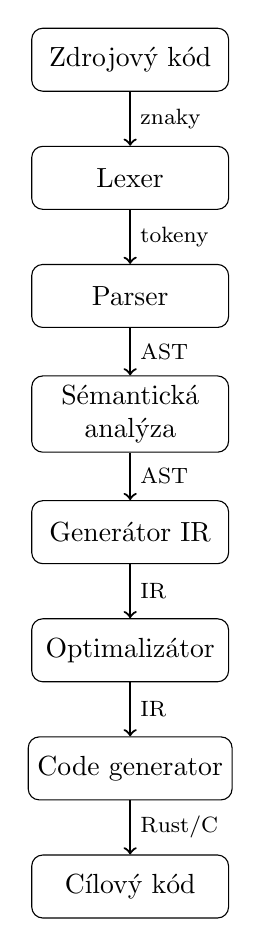
\begin{tikzpicture}[
			node distance=1.5cm,
			box/.style={rectangle, draw, rounded corners, minimum width=2.5cm, minimum height=0.8cm, align=center},
			arrow/.style={->, thick}
		]
		\node[box] (source) {Zdrojový kód};
		\node[box, below of=source] (lexer) {Lexer};
		\node[box, below of=lexer] (parser) {Parser};
		\node[box, below of=parser] (semantic) {Sémantická\\analýza};
		\node[box, below of=semantic] (ir) {Generátor IR};
		\node[box, below of=ir] (opt) {Optimalizátor};
		\node[box, below of=opt] (codegen) {Code generator};
		\node[box, below of=codegen] (target) {Cílový kód};

		\draw[arrow] (source) -- (lexer) node[midway, right] {\footnotesize znaky};
		\draw[arrow] (lexer) -- (parser) node[midway, right] {\footnotesize tokeny};
		\draw[arrow] (parser) -- (semantic) node[midway, right] {\footnotesize AST};
		\draw[arrow] (semantic) -- (ir) node[midway, right] {\footnotesize AST};
		\draw[arrow] (ir) -- (opt) node[midway, right] {\footnotesize IR};
		\draw[arrow] (opt) -- (codegen) node[midway, right] {\footnotesize IR};
		\draw[arrow] (codegen) -- (target) node[midway, right] {\footnotesize Rust/C};
	\end{tikzpicture}
	\caption{Fáze kompilátoru \Roth{}}
	\label{fig:compiler-pipeline}
\end{figure}


\subsubsection{Mezikód}
\label{sec:mezikod}

Mezikód (intermediate representation, IR) je klíčovou součástí
moderních kompilátorů. Odděluje frontend (analýza zdrojového kódu)
od backendu (generování cílového kódu), což umožňuje nezávislý
vývoj obou částí a~podporu více cílových platforem.

\paragraph{Typy mezikódu.}
Existuje několik základních typů mezikódu \autocite{aho2006}:

\begin{description}
	\item[Tříadresový kód] --- instrukce mají tvar \texttt{x = y op z},
	      kde každá instrukce má nejvýše tři operandy. Tento typ je
	      blízký instrukcím RISC procesorů.

	\item[SSA forma] (Static Single Assignment) --- varianta
	      tříadresového kódu, kde každá proměnná je přiřazena právě
	      jednou. SSA zjednodušuje mnoho optimalizací, zejména analýzu
	      datového toku.

	\item[Zásobníkový kód] --- instrukce pracují s~implicitním
	      zásobníkem, podobně jako bajtkód JVM nebo WebAssembly.
	      Tento typ je přirozený pro zásobníkové jazyky.

	\item[Graf toku řízení] (Control Flow Graph, CFG) --- program
	      je reprezentován jako orientovaný graf, kde uzly jsou
	      základní bloky a~hrany reprezentují možné přechody mezi nimi.
\end{description}

\paragraph{Mezikód kompilátoru Roth.}
Kompilátor \Roth{} používá zásobníkový mezikód, který přirozeně
odpovídá sémantice zdrojového jazyka. Každá instrukce IR popisuje
operaci nad datovým zásobníkem a~je anotována svým \emph{stack effect}
--- počtem hodnot, které odebírá ze zásobníku, a~počtem hodnot,
které na zásobník ukládá.

IR programu v~kompilátoru \Roth{} se skládá z~následujících
komponent:
\begin{itemize}
	\item \textbf{IRProgram} --- reprezentuje celý program, obsahuje
	      hlavní funkci a~slovník uživatelských funkcí.
	\item \textbf{IRFunction} --- reprezentuje jednu funkci (slovo),
	      obsahuje seznam instrukcí a~informaci o~stack effect.
	\item \textbf{IRInstruction} --- jednotlivá instrukce mezikódu.
\end{itemize}

Tabulka~\ref{tab:ir-instructions} uvádí přehled kategorií instrukcí
mezikódu.

\begin{table}[ht]
	\centering
	\caption{Kategorie instrukcí mezikódu}
	\label{tab:ir-instructions}
	\begin{tabular}{lll}
		\toprule
		\textbf{Kategorie} & \textbf{Příklady}    & \textbf{Popis}           \\
		\midrule
		Zásobníkové        & Push, Pop, Dup, Swap & Manipulace se zásobníkem \\
		Aritmetické        & Add, Sub, Mul, Div   & Aritmetické operace      \\
		Porovnávací        & Equal, Less, Greater & Relační operace          \\
		Logické            & And, Or, Not         & Booleovské operace       \\
		Řídicí tok         & Jump, JumpIf, Call   & Větvení a~volání         \\
		Paměťové           & Load, Store          & Práce s~proměnnými       \\
		I/O                & Print, ReadChar      & Vstup a~výstup           \\
		\bottomrule
	\end{tabular}
\end{table}


\subsubsection{Optimalizace}
\label{sec:optimalizace-teorie}

Optimalizace jsou transformace programu, které zachovávají jeho
sémantiku, ale zlepšují některou z~metrik kvality --- typicky
rychlost běhu nebo velikost kódu. Kompilátor \Roth{} implementuje
několik standardních optimalizačních technik.

\paragraph{Constant folding.}
Vyhodnocení konstantních výrazů v~době kompilace. Například
sekvence instrukcí \texttt{Push(5) Push(3) Add} může být nahrazena
jedinou instrukcí \texttt{LoadConst(8)}. Tato optimalizace je
zvláště účinná v~kombinaci s~inliningem.

\paragraph{Dead code elimination.}
Odstranění kódu, který nemá vliv na výsledek programu. Typickým
příkladem je hodnota uložená na zásobník, která je ihned odstraněna
bez použití: \texttt{Push(42) Drop} lze zcela eliminovat.

\paragraph{Peephole optimalizace.}
Lokální optimalizace, které hledají a~nahrazují krátké vzory
instrukcí efektivnějšími ekvivalenty. Příklady:
\begin{itemize}
	\item \texttt{Dup Add} $\rightarrow$ násobení dvěma
	\item \texttt{Swap Swap} $\rightarrow$ odstranění obou instrukcí
	\item \texttt{Push(a) Push(b) Swap} $\rightarrow$ \texttt{Push(b) Push(a)}
\end{itemize}

\paragraph{Strength reduction.}
Náhrada drahých operací levnějšími ekvivalenty. Například násobení
dvěma lze nahradit sečtením hodnoty se sebou samou (\texttt{Dup Add}),
což může být na některých platformách rychlejší než obecné násobení.

\paragraph{Function inlining.}
Nahrazení volání funkce jejím tělem. Inlining eliminuje režii
volání funkce a~umožňuje další optimalizace v~kontextu volajícího
kódu. Kompilátor \Roth{} provádí inlining pro malé funkce bez
řídicích struktur.

\paragraph{Iterativní optimalizace.}
Optimalizační průchody se typicky spouštějí opakovaně, dokud
se program stabilizuje (žádný průchod neprovede změnu). Jedna
optimalizace totiž může vytvořit příležitosti pro jinou. Například
inlining může vytvořit nové konstantní výrazy, které lze následně
zoptimalizovat pomocí constant foldingu.

Kompilátor \Roth{} implementuje optimalizační pipeline, která
spouští průchody v~definovaném pořadí:
\begin{enumerate}
	\item Function inlining --- nejdříve vložit těla funkcí
	\item Constant folding --- vyhodnotit konstantní výrazy
	\item Peephole optimalizace --- aplikovat lokální vzory
	\item Strength reduction --- nahradit drahé operace
	\item Dead code elimination --- odstranit mrtvý kód
\end{enumerate}

Pipeline se opakuje až do dosažení fixního bodu nebo maximálního
počtu iterací (standardně 10).
